
\chapter{Východzia situácia}\label{chap:intro} 
\section{Obchodovanie na menovej burze} 
\subsection{Menová burza} 
\begin{mydef} 
{\bf Burza}\cite{ZAC} je osobitný druh organizovaného trhu, na ktorom predávajúci a kupujúci uskutočňujú obchody istých zastupiteľných objektov. 
\end{mydef} 
Kedže sa sa rozprávame o menovej burze, zastupiteľské objekty sú meny. 
\subsection{Zarábanie na menovej burze} 
Na burze sa dá zarobiť spôsobom, že kúpite lacnejšie a predáte drahšie. Je to možné vďaka tomu, že na menovej burze kurz, cena za ktorú kúpite danú menu, nie je stály. A aké veľké sú výkyvy tohto kurzu, určuje volatilita burzy. 
\begin{mydef}
{\bf Volatilita}\cite{vlachy2006vrizeni} je smerodajná odchýlka výnosu trhovej hodnoty podniku alebo rizikového faktoru. 
\end{mydef} 
Inak povedané volatilita je kolísanie. Miera neistoty. Spravidla platí, že čím vyššie výnosy, tým vyššia volatilita. 
\subsubsection{Vysoká volatilita} 
\begin{figure}[!hbt] 
\begin{center} 
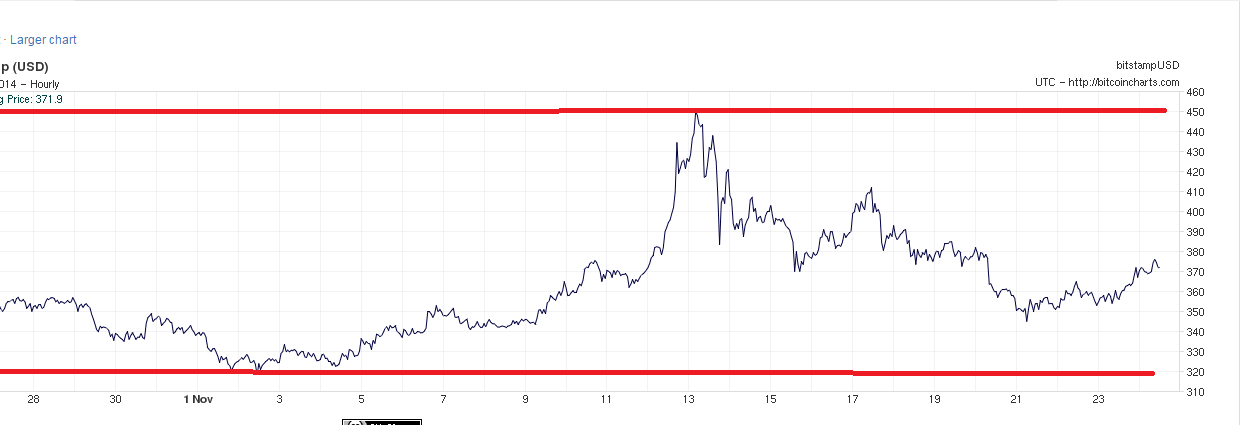
\includegraphics[width=1\textwidth]{obr} 
\caption{Vysoká volatilita} 
\label{img:vvolat} 
\end{center} 
\end{figure} 
\begin{myex}
Na obrázku \ref{img:vvolat}  vidíme vysoko volatilnú burzu, ktorou je bitcoin a USD. Možný zisk sa pohybuje až na úrovni 37,5 percenta za mesiac, keď nerátame poplatky. V prvom obrázku je jeden dielik 10 dolárov.  
\end{myex}
\subsubsection{Nízka volatilita}  
\begin{figure}[!hbt] 
\begin{center} 
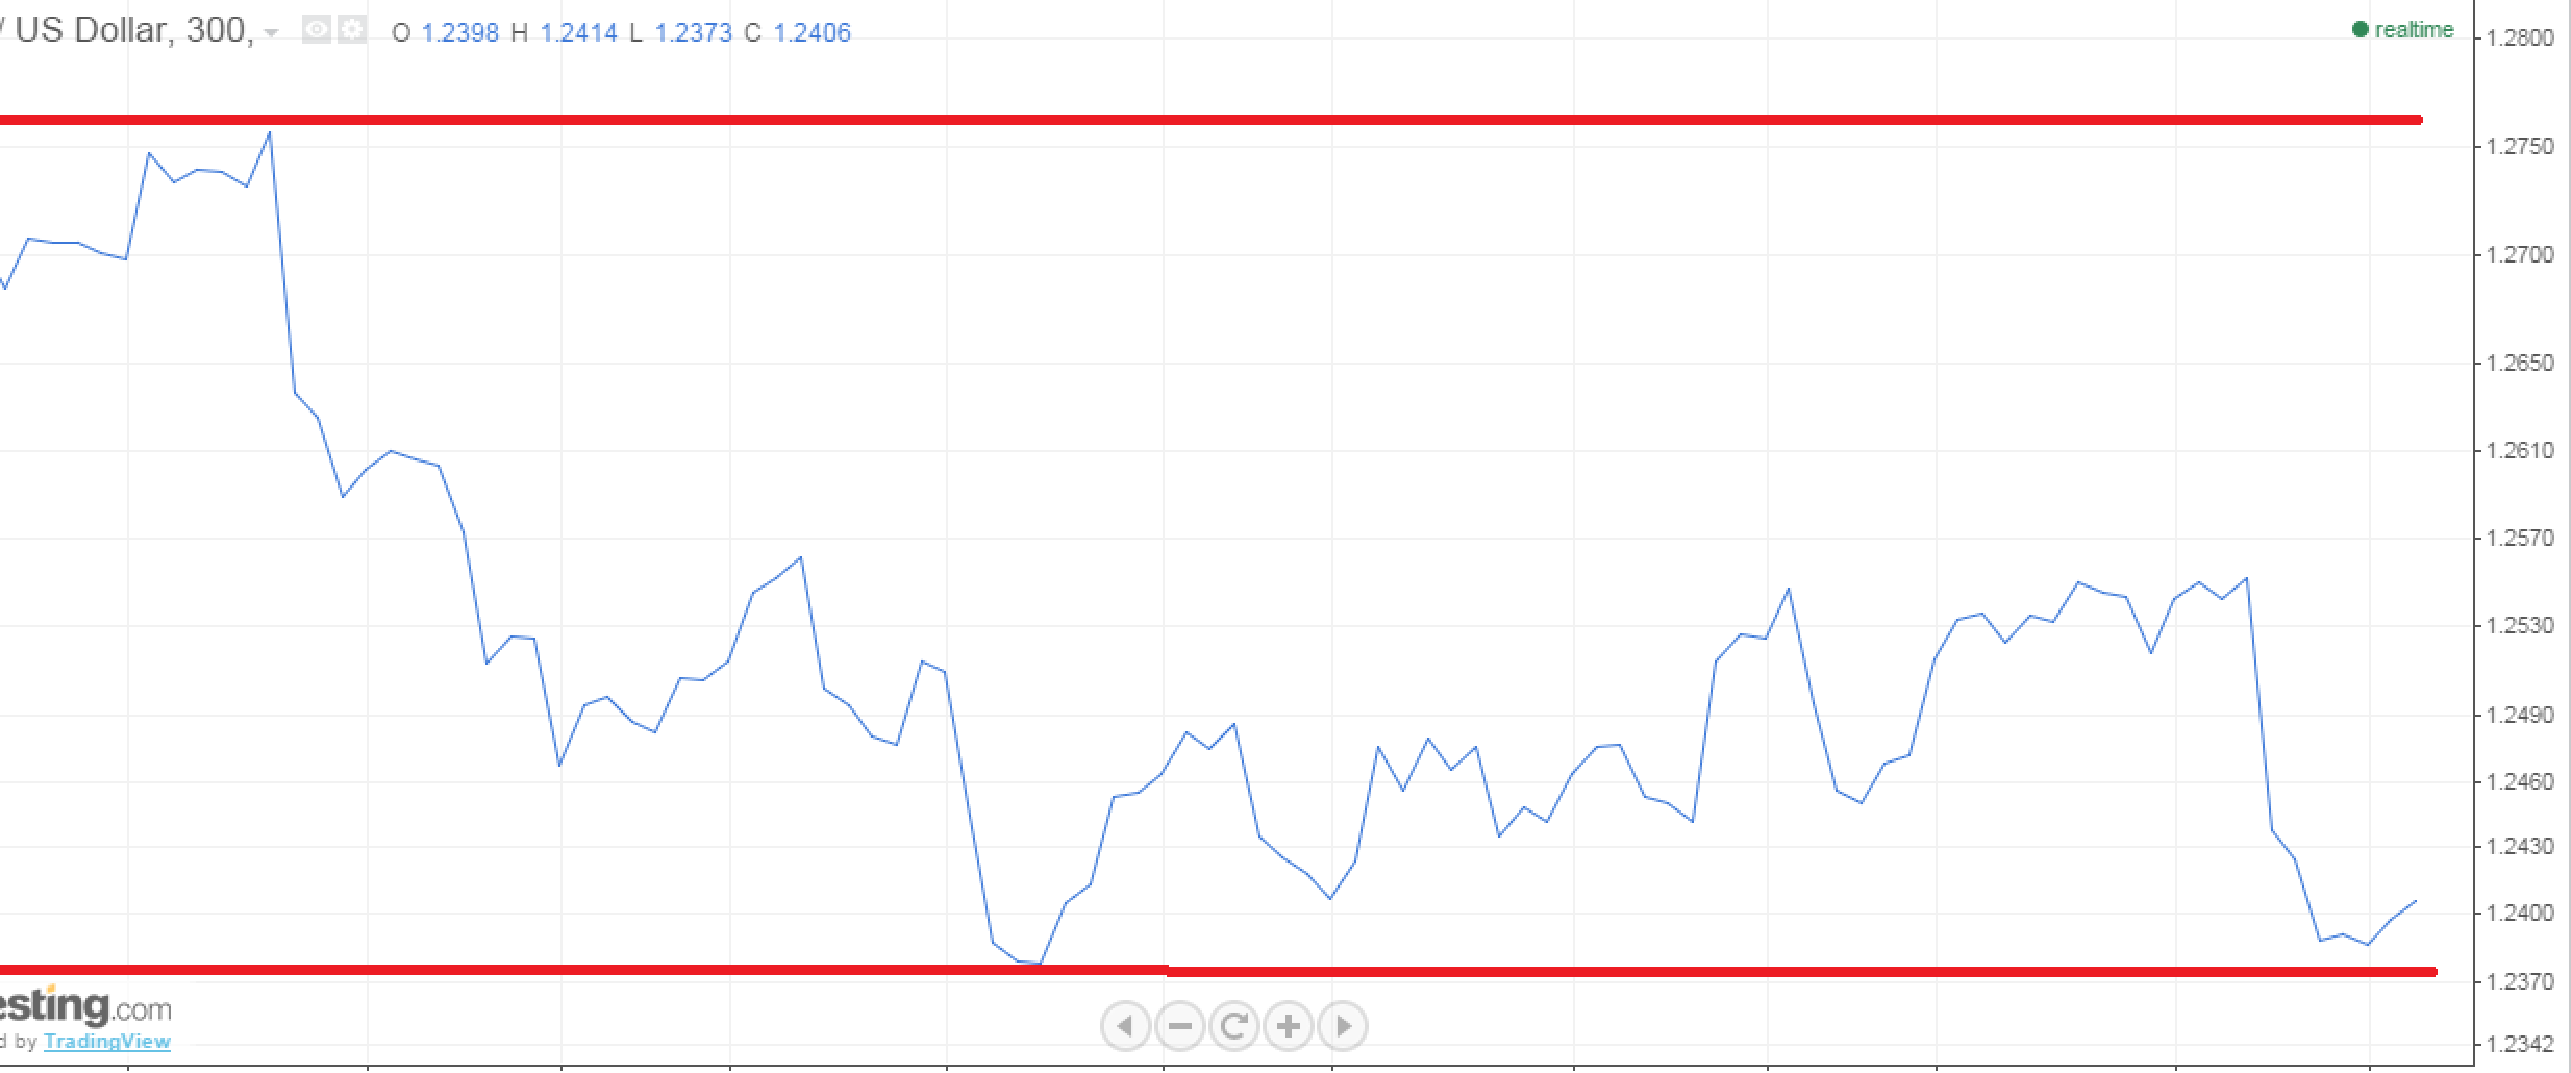
\includegraphics[width=1\textwidth]{obr2} 
\caption{Nízka volatilita} 
\label{img:nvolat} 
\end{center} 
\end{figure} 

\begin{myex}
Obrázok \ref{img:nvolat} ukazuje zmeny kurzu z málo volatilnej burzy, kde je  možný zisk iba 2,95 percenta za mesiac a jeden dielik je tisícina danej meny.   
\end{myex} 


\subsubsection{Broker} 
\begin{mydef} 
{\bf Broker}\cite{ZAC} je spoločnosť, ktorá má uzavreté dohody s burzami ohľadne prístupu na ne a poskytovanie dát z nich.
\end{mydef} 
Vy sami ako malí investori sa nemôžete dohodnúť s burzou, že u nej budete obchodovať alebo že vám bude zasielať historické dáta. O to sa postará broker, ktorý je dosť veľký na to aby s ním burza uzavrela obchody a oplatilo sa jej to. Taktiež môže slúžiť ako investor. To znamená, že niekoľko krát znásobí náš vklad aby naše zisky boli niekoľko krát väčšie. Samozrejme dáva pozor aby sme nestratili jeho peniaze, a ak by sme mali klesnúť pod hranicu jeho peňazí zakáže nám ďalej obchodovať.  
\section{Okrajové burzy} 
Keďže chceme obchodovať bez brokera, vyhovujú nám okrajové burzy. 
\subsection{Výhody} 
Medzi výhody okrajových búrz patrí aj vysoká volatilita, ktorú som predstavil vyššie. 
\subsubsection{Absencia \uv{Veľkých hráčov}} 
Veľký hráči\cite{ZAC} sú hlavne veľké korporácie a bohatí investori. Za to my sme na trhu malí hráči, lebo máme malý kapitál. Na okrajových burzách nie sú veľkí hráči kvôli tomu, že táto burza má ponuky s nízkym kapitálom a na ich investíciách by sa vysoko prejavila likvidita. Pojem likvidity vysvetlím v nevýhodách. 
\subsubsection{Nízke poplatky} 
Výhodou okrajových búrz sú nízke transakčné a iné poplatky. Transakčné poplatky sa pohybujú od 0,1 percenta z transakcie. Na veľkých burzách treba ku vyšším poplatkom prirátať ešte poplatok pre brokera.
\subsection{Nevýhody} 
\subsubsection{Veľká likvidita trhu} 
\begin{mydef} 
{\bf Spread}\cite{ZAC} je rozdiel medzi ponukou a dopytom.
\end{mydef} 
Ak je ponuka 1,5 a dopyt 1,6 spread je 0,1.
\begin{mydef} 
{\bf Trhová likvidita}\cite{revzvnakova2007mezinarodni} ako stupeň či miera, do ktorej môže podnik emitovať zastupiteľské objetky, bez toho, aby klesla trhová cena existujúceho zastupiteľského objektu, je determinovaná nielen dopytom investorov, ale aj ponukovou stranou z hľadiska charakteristík každého podniku. 
\end{mydef}
\begin{figure}[!hbt] 
\begin{center} 
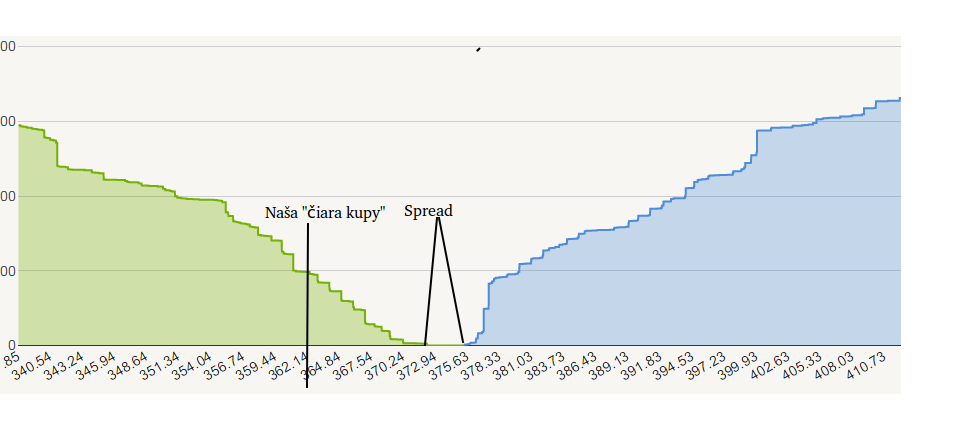
\includegraphics[width=1\textwidth]{stamp} 
\caption{\uv{Order book} na Bitstamp-e} 
\label{img:ob} 
\end{center} 
\end{figure} 
  Likvidita trhu vyjadruje zmenu ceny pri obchodoch. Ak je likvidita nízka, tak veľké investície dočasne výrazne zmenia kurz a naopak, ak je likvidita vysoká, veľké obchody kurz zmenia minimálne. Súvisí to s tým, aké veľké množstvo peňazí je na burze. Trh na obrázku \ref{img:ob} má nízku likviditu. Vidíte ponuku, dopyt a spread. Ak chce niekto spraviť obchod za väčšie množstvo peňazí, len malé percento zo sumy kúpi za aktuálny kurz, lebo nie je dostatočný počet ponúk s takouto cenou. Zvyšok kupuje stále za drahšie, až príde po miesto, kt. na obrázku vyznačujem ako \uv{čiara kúpy}. Do času reakcie trhu vznikne obrovský spread a tiež to výrazne ovplyvní kurz. Preto sa veľkým hráčom sa neoplatí obchodovať na okrajových burzách. 
\subsubsection{Väčšie riziko} 
Na okrajových burzách je väčšie riziko, že svoje investície stratíte bez vášho pričinenia. Môže sa totiž stať, že burza za noc ukončí svoje pôsobenie a prestane odpovedať. V nedávnej minulosti sa stalo, že významné okrajové burzy zo dňa na deň zmizli a ľudia prišli o svoje investície.  
\subsection{Zhrnutie} 
Z toho čo som spomenul predtým je zjavné,  že pre naše zámery je okrajová burza ideálna. Keďže naše investície do burzy nie sú veľké, veľkými výhodami sú pre nás nízke poplatky a absencia veľkých hráčov, pričom vysoká likvidita je pre nás iba malou nevýhodou. S ostatnými rizikami a nevýhodami musíme rátať. Ktoré burzy(platformy) vyhovujú našim požiadavkám uvediem potom ako predstavím pojem algoritmického obchodovania a menu ktorá sa na týchto burzách vyskytuje. 
\section{Algoritmické obchodovanie} 
Algoritmus je špecifická množina jasne definovaných inštrukcií, ktorých cieľom je vykonať úlohu alebo proces. \\ 
Algoritmické obchodovanie (automatizované obchodovanie, obchodovanie black-box, alebo jednoducho algo obchodovanie) je proces používania počítačov, naprogramovaných nasledovať definovaný algoritmus, ktorý je usmernený na vykonanie obchodu s cieľom vytvárať zisk, a to s  rýchlosťou a frekvenciou, ktoré sú nemožné pre človeka - obchodníka. Deje sa tak v definovanej sade pravidiel, ktoré sú založené na načasovaní, cene a iných kritériách. Okrem ziskovej príležitosti pre obchodníka je algo-obchodovanie %na trh likvidnejšie a 
robí obchodovanie systematickejšie vylúčením emocionálneho vplyvu človeka na obchodné činnosti.\cite{Ba} \\ 
Aby mohlo prebiehať algoritmické obchodovanie musí mať burza API. API je prístup pre algoritmus na burzu. 
\subsection{Backtesting} 
Backtesting je spôsob ako otestovať svoj algoritmus. Používajú sa historické dáta z búrz na otestovanie účinnosti algoritmu. 
\section{Bitcoin} 
V poslednej dobe sa výrazne zvýšil počet búrz s takzvanými \uv{krypto menami} a jednou z najvýznamnejších je práve bitcoin. 
\subsection{O bitcoine} 
Bitcoin umožňuje nový platobný systém s úplne digitálnymi peniazmi. Jedná sa o prvú decentralizovanú platbu siete \uv{peer-to-peer}, ktorá je poháňaná svojim užívateľom bez ústredného orgánu alebo sprostredkovateľov. Z užívateľského hľadiska je používanie bitcoinu skoro také jednoduché ako používanie internet bankingu. Bitcoin je prvá realizácia koncepcie nazvanej \uv{krypto meny}, ktorá bola prvýkrát popísaná v roku 1998 pánom Wei Dai a naznačovala myšlienku novej formy peňazí, ktorá používa šifrovanie na riadenie jej vzniku a transakcií, miesto centrálnych autorít.  Prvá špecifikácia bola publikovaná v roku 2009  Satoshi Nakamotom. 
\subsection{Spôsob získavania} 
Bitcoini môžete získať viacerými spôsobmi. Môže vám niekto nimi zaplatil, môžete ich kúpiť na burze alebo ich jednoducho dostanete. Ale existuje ešte jeden zaujímavý spôsob a to je ťažba. 
\subsubsection{Ťažba} 
Toto je spôsob, keď požičiate výpočtovou kapacitu svojho zariadenia na vedecké účely a za odmenu získate istý počet bitcoinov. 
 Sprostredkovatelia sú napríklad  Cgminer, Guiminer a BAMT. Mh/s je jednotka určujúca výpočtový výkon. Ukazuje koľko je vaše ťaženie schopné urobiť operácií za jednu sekundu. Platí, že čím viac, tým väčší zisk. 
\subsection{Použitie} 
Bitcoin sa už v hojnej miere používa na internete. Podporuje ho už aj veľa známych obchodov. Dokonca už niektoré ne-internetové obchody zaviedli platenie bitcoinami. Na Slovensku máme už aj bitcoinový bankomat. 
 \\ 
Bohužiaľ, keďže bitcoin je slabo kontrolovateľný, často sa využíva na nelegálne obchody s drogami alebo na pranie peňazí. \cite{B} 
\section{Vyhovujúce platformy} 
Ako som spomenul pri algoritmickom obchodovaní, potrebujeme aby burza mala svoje API. V tejto časti si predstavíme burzy, ktoré najviac vyhovujú naším požiadavkám. Sú to burzy s krypto-menami a hlavne s bitcoinom, lebo ten má pre nás veľmi dobré vlastnosti. 
\subsubsection{BITSTAMP} 
Túto burzu preferujeme najviac a na tejto burze chceme začať. Moja bakalárska práca sa pravdepodobne bude týkať hlavne tejto burzy. BITSTAMP ma veľmi prehľadné API, vyhovujúce transakčné poplatky a iné nám vyhovujúce vlastnosti. Transakčné poplatky sú od 0,5 percenta z transakcie, keď je transakcia do 500 dolárov až po 0,2 percenta keď je naša transakcia nad 120000 dolárov. Obchodovací pár je BTC/USD. \cite{Bit} 
\subsubsection{Bitfinex} 
Tu sa poplatky pohybujú od 0,1 až po 0,2 percenta z transakcie. Obchodovací pár je BTC/USD. Okrem bitcoinu sa dá obchodovať ešte z namecoinom a litecoinom. \cite{Bitf} 
\subsubsection{BTC-e} 
Poplatky sa transakciu sú od 0,2 do 0,5. Obchodovací pár je BTC/USD. \cite{BTC} 
\subsubsection{Kraken} 
Táto burza okrem bitcoinu obchoduje aj s inými krypto-menami, preto by sme túto burzu použili, keby by sme chceli prejsť na tieto meny. \cite{Kre} 
\section{Existujúce riešenie} 
\subsection{Tradewave} 
Toto existujúce riešenie vzniklo iba toto leto, tým pádom až potom ako sme začali rozvíjať našu myšlienku. Tradewave je veľmi podobný tomu, čo chceme vytvoriť my, dokonca v užívateľskom rozhraní je ešte lepší, má však niektoré, pre nás podstatné, nevýhody.  
\subsubsection{Čo je to Tradevawe?} 
Tradewave je veľmi pohodlný spôsob, ako si vytvoriť vlastní obchodovací algoritmus. Programátorský jazyk sa používa Python. Obchoduje práve na tých burzách, ktoré som spomínal v časti \uv{Vyhovujúce platformy}. Je kompletne automatizovaný. Obchody, grafy a záznamy zobrazuje v reálnom čase. Algoritmus môže bežať neustále na ich serveroch a tiež sa pohodlne spustiť a zastaviť. Dokonca má aj mailové upozorňovanie. Priamo na stránke Tradewave sa dá váš algoritmus aj jednoducho a rýchlo testovať na historických dátach.  \cite{Tw} 
\begin{figure}[!hbt] 
\begin{center} 
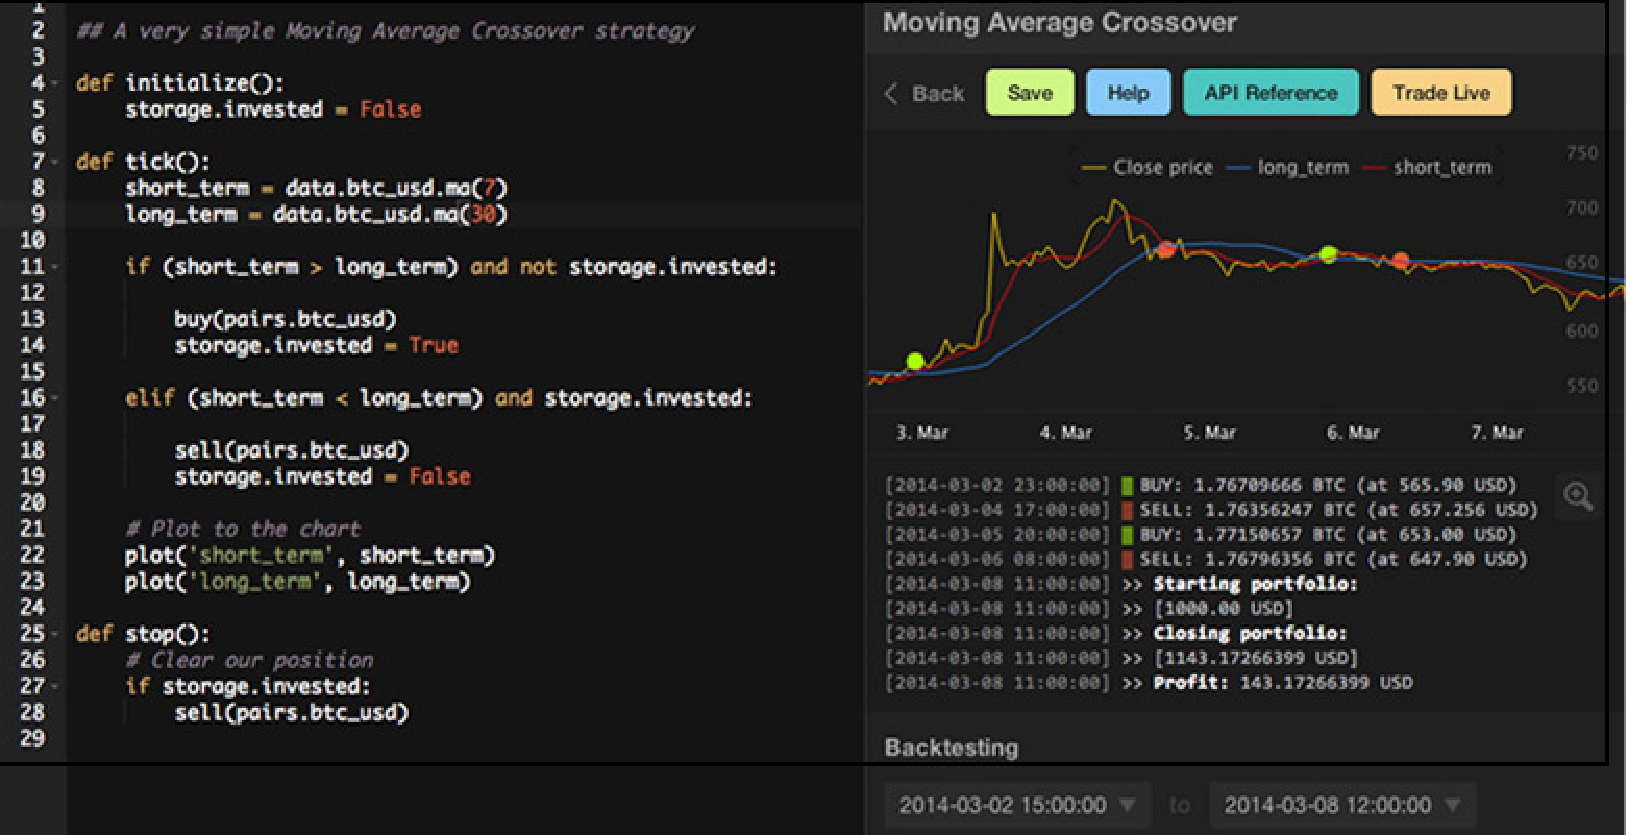
\includegraphics[width=1\textwidth]{trade} 
\caption{Tradewawe} 
\label{img:trade} 
\end{center} 
\end{figure} 
\ref{img:trade} 
\subsubsection{Vzhľadom k nášmu riešeniu} 
Toto riešenie je oproti nášmu veľmi užívateľský pohodlné. My sa nebudeme venovať užívateľskému rozhraniu, keďže s naším algoritmom a jeho testovaním budeme pracovať iba my. Ale nemôžme použiť nič z tohto existujúceho riešenia, pretože nemajú verejné kódy a hlavným dôvodom, prečo nemôžme Tradewave použiť je, že pri používaní tejto platformy sa všetko použité stáva aj ich vlastníctvom. Preto vzhľadom na fakt, že v budúcnosti by sme chceli na našom algoritme aj zarábať, si nemôžme dovoliť použiť Tradewave a tak odovzdať naše nápady a kódy niekomu inému. 
\section{Použité technológie} 
V tejto časti predstavíme technológie, ktoré budú použité pri programovaní algoritmu a testovania. 
\subsubsection{Ruby} 
Väčšina kódu bude naprogramovaná jazyku v Ruby. Ruby je dynamický, open source programovací jazyk so zameraním na jednoduchosť a produktivitu. Má elegantnú syntax, ktorú je prirodzene čítať a jednoducho písať. Ruby bol prvý krát uvedený v roku 1995 svojím tvorcom Yukihiro “Matz” Matsumoto. Matz skombinoval svoje obľúbené jazyky (Perl, Smalltalk, Eiffel, Ada, and Lisp). Ruby je vyvážením funkcionálneho a imperatívneho programovania. Svojej obľube sa teší až od roku 2006.\cite{Rb} 
\subsubsection{Python} 
Nejaké časti kódu sa môžu objaviť aj v jazyku Python. Python je interpretovaný, objektovo orientovaný, vysoko-úrovňový programovací jazyk s dynamickou sémantikou. Je postavený na dátových štruktúrach, v kombinácii s dynamickým písaním a dynamickými väzbami, aby bol atraktívny pre rýchly vývoj aplikácií. Rovnako môže byť použitý ako skriptovací jazyk alebo ako \uv{gloo language} na pripojenie existujúcich komponentov dohromady. Prvé uvedenie Pythonu je z decembra 1989 svojím tvorcom Guido van Rossum\cite{Pt} 
